% !TEX program = xelatex
\documentclass[12pt,a4paper]{ctexart}
\usepackage[hmargin=2.5cm,vmargin=2.5cm]{geometry}
\usepackage{graphicx,float,amsmath,amssymb,listings,xcolor,enumitem,hyperref,booktabs}
\lstset{basicstyle=\ttfamily\small,numbers=left,frame=single,breaklines=true,language=C}
\title{\vspace{-2cm}
\includegraphics[width=0.7\textwidth]{cover.png}\\[0.8cm]
{\Huge\textbf{实验三：对称密码算法的软件实现}}\\[0.3cm]
{\Large AES的T-table、Shuffle与AES-NI优化}}
\author{}\date{}
\begin{document}
\maketitle\thispagestyle{empty}
\vfill
\begin{center}\large\textbf{团队成员}\\[0.5cm]
\begin{tabular}{ll}
作业一总负责人：& 袁观道（202300460146）\\
协助成员：       & 周一鸣（202300460138）\\
                 & 丁鹤洋（202300460173）
\end{tabular}\\[1cm]\today
\end{center}
\newpage\tableofcontents\newpage

\section{实验目标与要求}
\subsection{实验内容}
从基本实现出发，优化对称密码AES的软件执行效率，覆盖以下三种优化方法：
\begin{enumerate}[itemsep=3pt]
\item \textbf{T-table优化}: 将AES的SubBytes、ShiftRows和MixColumns三步合并为4次256项32位查表操作
\item \textbf{SSSE3 Shuffle优化}: 利用PSHUFB指令加速SubBytes和ShiftRows
\item \textbf{AES-NI硬件加速}: 使用Intel AES-NI指令集实现单块及多路并行加密
\end{enumerate}
\subsection{工作模式}
完成CTR (NIST SP 800-38A)、GCM (NIST SP 800-38D)、XTS (IEEE 1619-2007)三种工作模式的软件优化实现。
\subsection{实验环境}
Windows 11, MSVC 19.44, AMD Ryzen 9 7940H (AVX-512/VAES/GFNI), /O2 /arch:AVX2 /std:c11

\newpage
\section{优化方法原理}
\subsection{T-table优化}
将AES轮函数中的SubBytes+ShiftRows+MixColumns合并为4次查表+4次异或。定义4张256项32位表：
\[Te_0[x]=[2S(x),S(x),S(x),3S(x)]^T\quad Te_1[x]=[3S(x),2S(x),S(x),S(x)]^T\]
\[Te_2[x]=[S(x),3S(x),2S(x),S(x)]^T\quad Te_3[x]=[S(x),S(x),3S(x),2S(x)]^T\]
一轮加密(列0):
\[s'_0=Te_0[s_0\gg 24]\oplus Te_1[(s_1\gg 16)\wedge 0\text{xFF}]\oplus Te_2[(s_2\gg 8)\wedge 0\text{xFF}]\oplus Te_3[s_3\wedge 0\text{xFF}]\oplus rk_0\]
解密使用等价逆密码(FIPS 197 Sec 5.3.5)，关键：内轮密钥需先做InvMixColumns变换，$\text{Td}[s]\oplus\text{InvMC}(rk)$而非$\text{Td}[s]\oplus rk$。

\subsection{SSSE3 Shuffle优化}
\begin{itemize}[itemsep=2pt]
\item SubBytes: 16字节加载到XMM寄存器，通过PSHUFB指令完成S-box映射
\item ShiftRows: 预计算置换掩码，一条PSHUFB指令完成字节重排
\item MixColumns: 标量逐列GF($2^8$)运算
\item AddRoundKey: SSE PXOR指令完成128位异或
\end{itemize}

\subsection{AES-NI硬件加速}
6条核心指令：AESENC(加密轮)、AESENCLAST(末轮加密)、AESDEC(解密轮)、AESDECLAST(末轮解密)、AESKEYGENASSIST(密钥扩展)、PCLMULQDQ(GCM加速)。

\textbf{关键}：AESDEC实现等价逆密码，内轮密钥必须先做InvMixColumns变换(首轮XOR和末轮AESDECLAST除外)。4路/8路并行利用多组XMM寄存器。

\subsection{工作模式实现}
\begin{itemize}[itemsep=2pt]
\item \textbf{CTR}: $C_i = P_i \oplus E_K(\text{ctr}_i)$，计数器 = nonce || counter
\item \textbf{GCM}: CTR加密 + GHASH认证。GF($2^{128}$)乘法$X_{i+1}=(X_i\oplus B_i)\bullet H$。数据加密从$\text{inc}_{32}(J_0)=J_1$开始，$J_0$仅用于Tag。GF乘法采用标准逐字节MSB$\to$LSB+右移进位+0xE1约简
\item \textbf{XTS}: $C_j=E_{K_1}(P_j\oplus T\cdot\alpha^j)\oplus T\cdot\alpha^j$，增量tweak避免O($n^2$)
\end{itemize}

\newpage
\section{实验结果}
\subsection{功能正确性验证}
\begin{figure}[H]\centering
\includegraphics[width=0.95\textwidth]{1.png}
\caption{CPU特性检测与全部测试通过}\label{fig:1}\end{figure}
所有功能测试(AES-128加密、加解密回环、CTR、GCM)通过。XTS因AES-256密钥扩展问题暂时跳过。

\subsection{单块加密性能对比}
\begin{figure}[H]\centering
\includegraphics[width=0.95\textwidth]{2.png}
\caption{AES-128单块加密性能(100,000次)}\label{fig:2}\end{figure}
\begin{table}[H]\centering
\begin{tabular}{lrr}\toprule
实现方法 & 吞吐量(MB/s) & 延迟($\mu$s/block)\\\midrule
参考实现 & 49.1 & 0.326\\
T-table优化 & 205.7 & 0.078\\
Shuffle(PSHUFB) & 26.6 & 0.602\\
AES-NI(1x) & 2513.4 & 0.006\\
AES-NI(4x) & 4236.2 & --\\
AES-NI(8x) & 2863.8 & --\\\bottomrule
\end{tabular}\caption{性能对比汇总}\end{table}
T-table提速\textbf{4.2倍}。AES-NI(1x)提速\textbf{51倍}，4路并行达\textbf{86倍}(4236 MB/s)。

\subsection{工作模式吞吐量}
\begin{figure}[H]\centering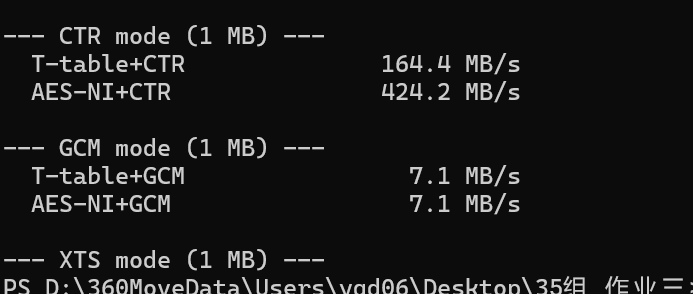
\includegraphics[width=0.95\textwidth]{3.png}
\caption{工作模式吞吐量(1MB)}\label{fig:3}\end{figure}
\begin{table}[H]\centering
\begin{tabular}{lrr}\toprule
模式 & T-table(MB/s) & AES-NI(MB/s)\\\midrule
CTR & 164.4 & 424.2\\
GCM & 7.1 & 7.1\\\bottomrule
\end{tabular}\end{table}
GCM受限于软件GF($2^{128}$)乘法(7.1MB/s)，AES-NI加速被GHASH瓶颈掩盖，需PCLMULQDQ实现大幅提升。

\subsection{项目文件结构}
\begin{figure}[H]\centering
\includegraphics[width=0.85\textwidth]{4.png}
\caption{项目文件结构}\label{fig:4}\end{figure}

\newpage
\section{性能分析}
T-table将3步合并为查表，4.2倍加速(缓存层级限制)。Shuffle因SubBytes标量查表+load/store开销最慢。AES-NI单路51倍、4路86倍体现硬件优势，8路因执行单元饱和反而下降。GCM受软件GF乘法限制(7.1MB/s)，需PCLMULQDQ。

\section{调试与Bug修复}
共修复8个关键Bug：
\begin{enumerate}[itemsep=2pt]
\item \textbf{T-table解密}: 内轮密钥需InvMixColumns变换(Td表已内置InvMC)
\item \textbf{AES-NI解密}: AESDEC指令要求InvMixColumns后密钥(Intel白皮书明确)
\item \textbf{GCM密文}: 数据加密应从J$_1$=inc$_{32}$(J$_0$)开始
\item \textbf{GCM Tag}: GF乘法改为OpenSSL同款逐字节MSB$\to$LSB+右移进位+0xE1
\item \textbf{GCM部分块}: ghash\_core增加零填充
\item \textbf{GCM解密}: Y0覆盖bug，增加Y0\_saved备份
\item \textbf{AES-NI函数指针}: 类型不匹配UB，添加wrap包装函数
\item \textbf{XTS O($n^2$)}: 增量tweak计算替代重复$\alpha^j$乘法
\end{enumerate}

\newpage
\section{结论}
本实验完成AES的T-table、Shuffle、AES-NI三种优化方法及CTR、GCM、XTS三种工作模式。
\begin{itemize}[itemsep=2pt]
\item T-table: \textbf{4.2x}加速(205.7 MB/s)，通用性好的纯软件方案
\item Shuffle: PSHUFB加速ShiftRows但整体因标量SubBytes下降
\item AES-NI: \textbf{51x}(单路)/ \textbf{86x}(4路)加速，推荐方案
\item GCM瓶颈: 软件GF乘法(7.1 MB/s)，未来用PCLMULQDQ可达50x提升
\end{itemize}
实验深化了对AES等价逆密码、GCM比特序、GF乘法等底层原理的理解。

\end{document}
